\documentclass{modernsimplecv}
% try out different fonts: classic, fira, raleway, chivo
\usepackage[utf8]{inputenc}
\usepackage[top=2cm, bottom=2cm, outer=0cm, inner=0cm, margin=1cm, a4paper]{geometry}

% ------------------------------------------------------------------------------------
% you can try out different fonts here by commenting the following lines in and out
% -----------------------------------------------------------------------------------
%\usepackage[default]{raleway}
%\usepackage[sfdefault]{FiraSans} %% option 'sfdefault' activates Fira Sans as the default text font\renewcommand*\oldstylenums[1]{{\firaoldstyle #1}}\normalfont
%\usepackage[familydefault,light]{Chivo} 
%\usepackage[sfdefault,light,condensed]{roboto}
%\usepackage[default]{cantarell}
\usepackage[sfdefault]{AlegreyaSans}


\usepackage{beuron}
\usepackage{setspace}

\usepackage{wallpaper}
\usepackage{mdframed}


%------------------------------------------------------------------ Variablen

\newlength{\rightcolwidth}
\newlength{\leftcolwidth}
\setlength{\leftcolwidth}{0.48\textwidth}
\setlength{\rightcolwidth}{0.47\textwidth}
%\addtolength{\wpYoffset}{2.5cm}
%\CenterWallPaper{1.0}{img/wallpaper.png}

%------------------------------------------------------------------
\title{Curriculum Vitae}
\author{Paul Brenker}
\date{August 2024}

\pagestyle{empty}
\begin{document}

\thispagestyle{empty}
%-------------------------------------------------------------



\tikz[remember picture,overlay] {%
\node[rectangle, fill=white, anchor=north, minimum width=\paperwidth, minimum height=5cm](header) at (current page.north){};%
}

\begin{minipage}[t]{0.21\textwidth}
\vspace{0pt} % Trick for alignment
%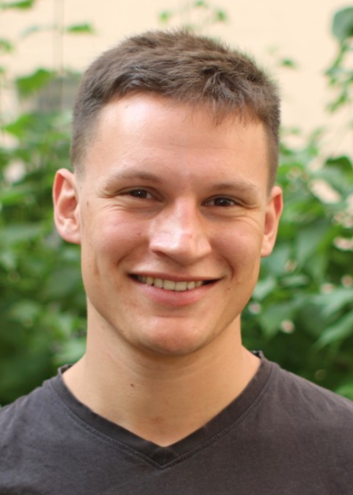
\includegraphics[width=\textwidth]{img/paul.png}\hspace{1em}
\end{minipage}
\hfill
\begin{minipage}[t]{1\textwidth}
\vspace{0pt} % Trick for alignment
\begin{shaded*}

\begin{minipage}[t]{0.47\textwidth}
\vspace{0pt} % Trick for alignment
% here the fancy font can be taken out by removing \LobsterTwo
{\par\centering\huge{Paul Brenker}} \\[0.3cm]
\faGlobe~ Nationality: German\\
\faBirthdayCake~ 1996 \\
\faMapMarker~ Bonn, Germany \\
\begin{spacing}{0.5}
{\small
\faCommentsO~ \underline{Languages:} 

  \begin{itemize}
    \item \emph{German} mother tongue
    \item \emph{English} full working proficiency
    \item \emph{Hebrew} limited working proficiency
    \item \emph{Arabic} basic knowledge
  \end{itemize}
}
\end{spacing}
\vspace{4pt} % Trick for alignment
\end{minipage}\hfill
\begin{minipage}[t]{0.46\textwidth}
\vspace{29pt} % Trick for alignment
\faPhone~ +49 173 5287524 \\
\faAt~ \protect\url{paul.brenker@gmail.com} \\

\faEnvelopeO~ Maxstr. 28, 53111 Bonn \\ 

%\aiAcademiaSquare 
\faGithub~ \protect\url{github.com/paulbrenker} \\
%\aiOrcid 
\faLinkedin~ \protect\url{linkedin.com/in/paul-brenker} \\
\end{minipage}
\hfill
\end{shaded*}
\end{minipage}\\[15pt]


%------------------------------------------------

\subsection*{}
\vspace{-3em}

\setlength{\columnsep}{1.7cm}
\columnratio{0.47}[0.46]
\begin{paracol}{2}
\hbadness5000


\paracolbackgroundoptions

% 0.9,0.9,0.9 -- 0.8,0.8,0.8


\small
\section*{Experience}

\begin{minipage}[t]{\leftcolwidth}
\begin{tabular}{r| p{0.6\textwidth} c}
    \cvevent{8/2023 - current}{SAP LeanIX}{Working Student}{Bonn, Germany}{integrated OpenAPI Specification evaluation tools for continuous integration pipelines. Contributed to the LeanIX EAM product as part of an agile engineering team. Learned to work with numerous technologies used in microservice architectures}{img/leanix_logo.jpg} \\

    \cvevent{2022-2023}{University of Bonn }{Student assistant}{Bonn, Germany}{Administration and maintenance of institute for philosophy websites and IT equipment.}{img/uni_bonn_logo.jpg} \\

    \cvevent{2017-2018}{Academy of Sciences and Humanities}{Student Assistant}{Berlin, Germany}{Transcription of ancient Hebrew and Arabic texts. XML annotation of academic text for cross-referenced usage in a database. Proofreading of articles.}{img/bbaw_logo.jpg}
\end{tabular}

\vspace{4em}

\begin{minipage}[t]{\leftcolwidth}
    \section*{Skills}
    \begin{tabular}{l l}
        \textbf{Java, Kotlin} & \textbf{Spring Boot}, Vaadin \\
        NodeJS & Nest \\
        Docker & \textbf{REST APIs}, GraphQL\\
        \textbf{Linux} & PostgreSQL \\
        Webdevelopment & Scrum \\
        Angular & LaTeX\\
        \textbf{Python} & Data Analysis \& Visualization \\
        Basic machine learning &  Clustering\\
    \end{tabular}
    \bigskip
    
\end{minipage}\hfill


\vspace{4em}
\end{minipage}
%-----------------------------------------------------------
\switchcolumn

\begin{minipage}[t]{\rightcolwidth}
\section*{Education}

\begin{tabular}{r| p{0.6\textwidth} c}
    \cvevent{2019 - 2024}{Bonn-Rhein-Sieg University of Applied Sciences (H-BRS)}{B.Sc Computer Science}{Bonn, Germany}{Finishing Computer Science degree in November 2024 with very good grades throughout the whole program. Specialized in Bioinformatics and Data Science. Thesis topic: Relevance of OpenAPI Linter Rules for Specification Quality.}{img/hbrs_logo.jpg} \\

    \cvevent{2015 - 2019}{Freie Universität zu Berlin}{B.A. History and Culture of the Middle East}{Berlin, Germany}{Language centered degree with long time abroad language courses in Egypt, Israel and Jordan. Thesis was written about gender-specific variations in the Arabic dialect of Amman, Jordan}{img/fu_logo.png} \\
\end{tabular}

\end{minipage}

\vspace{3em}

\begin{minipage}[t]{\leftcolwidth}
  \section*{Awards}
  \begin{tabular}{>{\small\bfseries}r >{\small}p{0.70\textwidth}}
      2023 & Deutschlandstipendium -  Scholarship for ambitious and talented students \\
      2018 & Scholarship for a full Semester of intensive Arabic language courses at the German Jordanian University in Amman, Jordan.\\
      2018 & PROMOS -  Scholarship for an intensive Hebrew summer school at the Ben Gurion University of the Negev \\
  \end{tabular}
  \bigskip
  
\end{minipage}\hfill

\bigskip

\begin{minipage}[t]{\rightcolwidth}
\section*{Volunteering}
\begin{tabular}{>{\small\bfseries}r >{\small}p{0.7\textwidth}}
    2014 & After graduating high school I volunteered for nine months in Kibbutz Ein Hashlosha in Israel. During my time I worked mostly in agriculture and landscaping but also in the local garage where I helped maintaining the tractors of the Kibbutz. \\
    
\end{tabular}
\bigskip

\section*{Hobbies}
\begin{tabular}{>{\small\bfseries}r >{\small}p{0.7\textwidth}}
    Rowing & I row since I am ten years old and participated in countless competitions including the german national sprint league. \\
    Cooking & My great passion is to cook. My favorite cuisines are Mediterranean and Asian.
\end{tabular}
\end{minipage}









\end{paracol}

\vfill{} % Whitespace before final footer

%----------------------------------------------------------------------------------------
%	FINAL FOOTER
%----------------------------------------------------------------------------------------
\setlength{\parindent}{0pt}
\begin{minipage}[t]{\textwidth}
\begin{center}\fontfamily{\sfdefault}\selectfont \color{black!70}
{\small Paul Brenker \icon{\faEnvelopeO}{black}{} Maxstr. 28 \icon{\faMapMarker}{black}{} 53111 Bonn \icon{\faPhone}{black}{} +4901735287525 
\icon{\faAt}{black}{} \protect\url{paul.brenker@gmail.com}
}
\end{center}
\end{minipage}
\end{document}